\documentclass[10pt,twocolumn,letterpaper]{article}

\usepackage{cvpr}
\usepackage{times}
\usepackage{epsfig}
\usepackage{graphicx}
\usepackage{amsmath}
\usepackage{amssymb}

% Include other packages here, before hyperref.

% If you comment hyperref and then uncomment it, you should delete
% egpaper.aux before re-running latex.  (Or just hit 'q' on the first latex
% run, let it finish, and you should be clear).
\usepackage[breaklinks=true,bookmarks=false]{hyperref}

\cvprfinalcopy % *** Uncomment this line for the final submission

\def\cvprPaperID{****} % *** Enter the CVPR Paper ID here
\def\httilde{\mbox{\tt\raisebox{-.5ex}{\symbol{126}}}}

% Pages are numbered in submission mode, and unnumbered in camera-ready
%\ifcvprfinal\pagestyle{empty}\fi
\setcounter{page}{4321}
\begin{document}

%%%%%%%%% TITLE
\title{Scene classification with Convolutional Neural Networks}

\author{Josh King\\
{\tt\small jking9@stanford.edu}
\and
Vayu Kishore\\
{\tt\small vayu@stanford.edu}
\and Filippo Ranalli\\
{\tt\small franalli@stanford.edu}
% For a paper whose authors are all at the same institution,
% omit the following lines up until the closing ``}''.
% Additional authors and addresses can be added with ``\and'',
% just like the second author.
% To save space, use either the email address or home page, not both
}

\maketitle
%\thispagestyle{empty}

%%%%%%%%% ABSTRACT
%\begin{abstract}
%The abstract is required and contains a 1-2 sentence summary of each section of the paper.
%\end{abstract}

%%%%%%%%% BODY TEXT
\section{Introduction}

We investigate the problem of \textit{scene classification}, in which scenes
from photographs are categorically classified. Unlike object classification, which
focuses on classifying prominent objects in the foreground, scene
classification uses the layout of objects within the scene, in addition to the
ambient context, for classification. The study of scene classification predates
the use of convolutional neural networks (CNNs), where, for example, previous
techniques include the use of
codebooks and bag-of-word models.\cite{Rasiwasia}\\

In this paper, we examine using supervised learning to train convolutional
neural networks to categorize scenes into a predefined set of categories.\\

%\section{Related Work}
%\cite{Zhou}
%\cite{Lin}
%\cite{Wu}

\section{Problem Statement}

We investigate how to train a CNN that can classify scenes with high Top-1
and Top-5 accuracy. We use the Places365-Standard scene dataset, which contains
365 categories with 1.6 million labelled images in the training set, 50 images
per category in the validation set, and 900 images per category in the test set
\cite{Zhou}.\\

\begin{figure}[h]
\begin{center}
  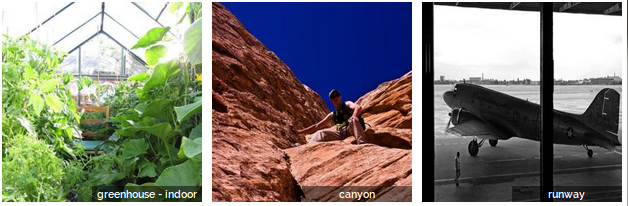
\includegraphics[width=0.8\linewidth]{places2db-cropped.png}
\end{center}
   \caption{Sample labelled images from the Places2 dataset}
\label{figure:sample-images}
\end{figure}


However, the test set provided is unlabelled. To evaluate our performance on
the test set, we will submit our model's labels to the Places365 evaluation
server, which will calculate our Top-1 and Top-5 accuracy. Additionally, the
validation data contains only the top label, so we can only evaluate the Top-1
accuracy during cross-validation.\\

In addition, through our exploration of training CNN's for this purpose, we
seek to learn if there are certain neural net features that result in good
performance for scene classification.\\

\subsection{Dataset Processing}
While we use the entire Places365-Standard dataset, we reduce the resolution of
the 256x256 images to 64x64 to allow us to run the images without running out of
memory on a Google Cloud Instance.\\

\section{Technical Approach}
We train existing CNN's such as ResNet\cite{ResNet}, and GoogLeNet on the
dataset. We will then tweak the architecture of the CNN's to see if we can
introduce features that will improve performance for scene classification. \\

In particular, for this report, we have trained the ResNet architecture, which
utilizes residual modules which learn residuals between the output of a set of
layers and their input. We implement the architecture described in
\cite{ResNet} using TensorFlow.  Additionally, as suggested in \cite{ResNet},
in order to allow a residual layer to span convolutional layers with multiple
dimensions, we zero-pad the output of the layers to maintain a consistent size.
To verify the correctness of our model, we overfit 100 samples.\\

\section{Preliminary Results}

We started by training a 34-layer ResNet written in Tensorflow on the entire
downsampled training dataset, validating against the validation set. To train
this, we used the hyperparameters outlined in Table \ref{table:hyper}. Major
architectural aspects of our design are described in Table \ref{table:arch}.
``Residual Layer Span'' describes the number of convolutional layers that the
residual layer learns residuals over. \\

As shown in Figure \ref{fig:top1-resnet34}, our preliminary model, with no
tuning and initialized to random weights before training obtains over 30\%
accuracy on the validation set. We expect further refinement of this model to
allow us to boost this further. The leaderboard of the Places365-Standard dataset
currently reports a 50\% best Top-1 accuracy. We also trained a smaller,
18-layer ResNet (shown in Figure \ref{fig:top1-resnet18} and Table \ref{table:acc18}), for
which we obtained similar results, with
a training accuracy of around 60\%, and a validation accuracy of 36\% .\\

\begin{table}
\begin{center}
\begin{tabular}{|l|c|}
\hline
Architecture & Description \\
\hline\hline
Loss & Softmax\\
Optimizer & Adam\\
Residual Layer Span & 2 \\
\hline
\end{tabular}
\end{center}
\caption{Description of ResNet architecture used for preliminary run}
\label{table:arch}
\end{table}

\begin{table}
\begin{center}
\begin{tabular}{|l|c|}
\hline
Hyperparameter & Value \\
\hline\hline
Minibatch size & 100 \\
Learning Rate & $10^{-4}$\\
Gradients Clipped to & 5\\
\hline
\end{tabular}
\end{center}
\caption{Description of ResNet hyperparameters used for preliminary run}
\label{table:hyper}
\end{table}

\begin{figure}[t]
\begin{center}
  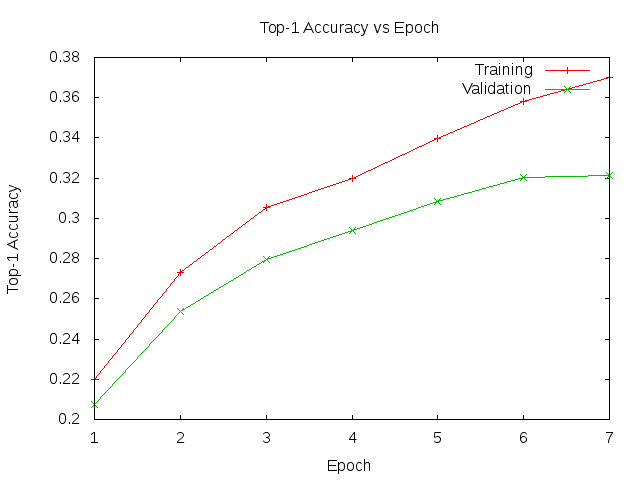
\includegraphics[width=0.8\linewidth]{accuracy_resnet34}
\end{center}
   \caption{Top-1 Training Accuracy vs Epoch for 34-Layer ResNet}
\label{fig:top1-resnet34}
\end{figure}

\begin{table}
\begin{center}
\begin{tabular}{|l|c|}
\hline
Training & Validation \\
\hline\hline
$59.66$ & $37.47$\\
\hline
\end{tabular}
\end{center}
\caption{Top-1 Accuracy for 34-Layer ResNet after 10 training epochs}
\label{table:acc}
\end{table}

\begin{figure}[t]
\begin{center}
  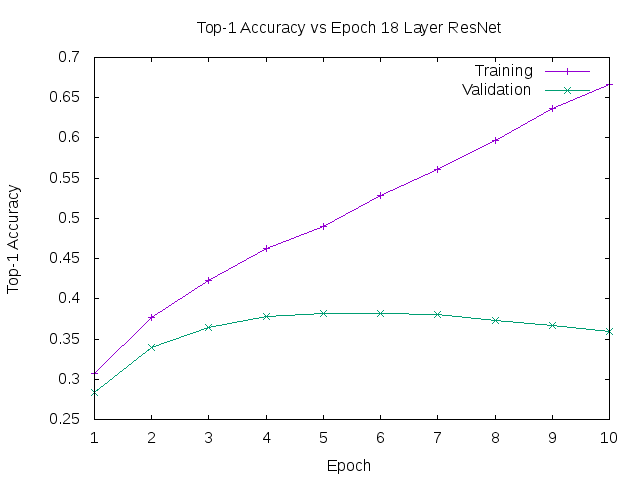
\includegraphics[width=0.8\linewidth]{accuracy_resnet18}
\end{center}
   \caption{Top-1 Training Accuracy vs Epoch for 18-Layer ResNet}
\label{fig:top1-resnet18}
\end{figure}

\begin{table}
\begin{center}
\begin{tabular}{|l|c|}
\hline
Training & Validation \\
\hline\hline
$66.4$ & $35.90$\\
\hline
\end{tabular}
\end{center}
\caption{Top-1 Accuracy for 18-Layer ResNet after 10 training epochs}
\label{table:acc18}
\end{table}

\section{Discussion}

Based on our results, though we perform well on the test set, our performance
on the validation set is much lower due to overfitting. To address this, we
will try tuning the learning rate further. In addition, we also noticed that
our validation accuracy decreased during our later training epochs while the
training accuracy continued to rise. To address this, we will add an early stop
to terminate training. Furthermore, we expect to obtain stronger results after tuning other hyperparameters within the CNN's.\\

\section{Future Work}

Future avenues of exploration include applying transfer learning by using
CNN's with pre-trained weights for object classification, and retraining the
final set of fully connected layers on the scene classification dataset.\\

Futhermore, we plan on visually examining misclassified images, to
gain more insight into reasons why our CNN's may be unable to categorize them properly.\\

Finally, if time permits, we will explore an ablation study of our models to
evaluate if there are certain characteristics of a CNN that allows it to perform
well on scene classification.\\


\nocite{Lin}
\nocite{Wu}


{\small
\bibliography{milestone}
\bibliographystyle{ieee}
}

\end{document}
